\documentclass[12pt]{article}


\usepackage[dvips,letterpaper,margin=0.75in,bottom=0.75in]{geometry}
\usepackage{cite}
\usepackage{slashed}
\usepackage{graphicx}
\usepackage{amsmath}

\usepackage[american,fulldiode]{circuitikz}

\begin{document}
\ctikzset{bipoles/thickness=1}
\ctikzset{bipoles/length=.6cm}

\title{Introduction to the Arduino} 

\maketitle

\section{Introduction}

\begin{figure}[htbp]
\begin{center}
 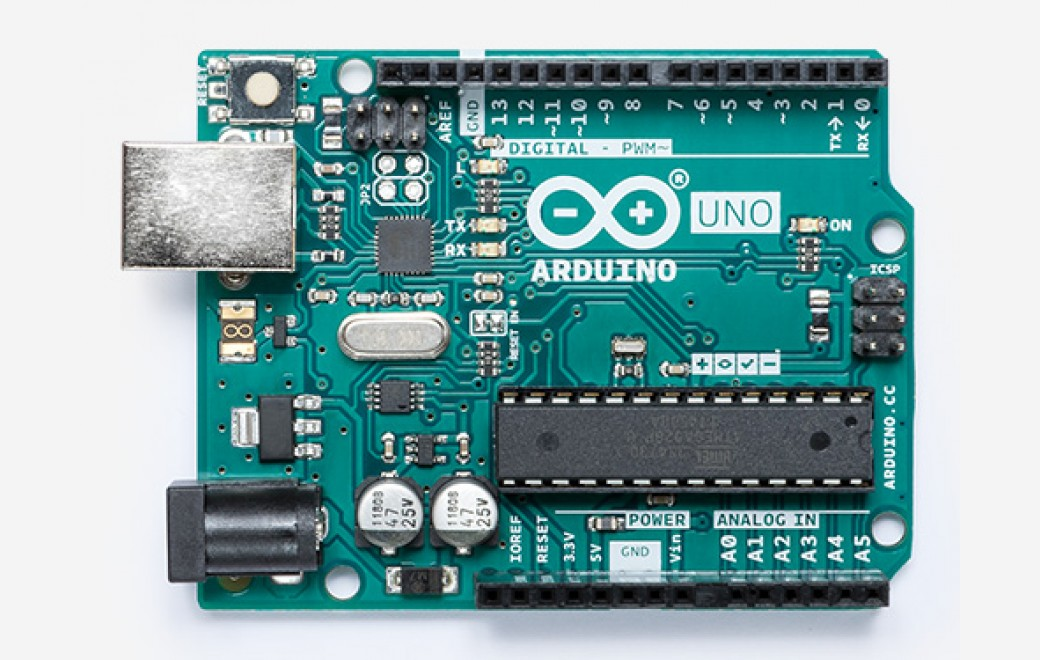
\includegraphics[width=0.55\textwidth]{figs/uno.jpg};
\caption{\label{fig:uno} The Arduino Uno microprocessor.}
\end{center}
\end{figure}

In this lab, we will learn to use the Arduino microprocessor, which we
will be using throughout the course to collect experimental data.  The model we will
use is the Arduino Uno.  The Arduino Uno is fairly robust and
inexpensive, so you should definitely be comfortable to experiment
with them.  However, to avoid the potential to damage the boards, you
should *NOT* supply any external power to the Arduino (e.g. from your
proto-board PB-503, bench-top power supply, or function generator.)

\section{The Arduino}

\noindent
{\bf Step 1:} The main Arduino website, which includes lots of
supporting documentation, is located at {\tt http://arduino.cc}.
Acquaint yourself with this site. 
\vspace{0.5 cm}

\noindent
{\bf Step 2:} The lab PCs have the Arduino software installed, and
each team will have an Arduino to work with.  Follow the instructions
for using the ``Arduino Desktop IDE" located here:  
{\tt https://www.arduino.cc/en/Guide/ArduinoUno}.
\vspace{0.5 cm}

\noindent
{\bf Step 3:} Adjust the pattern of the LED blink example to a slower rate. 
\vspace{0.5 cm}

\noindent
{\bf Step 4:}  The Arduino tutorials and built-in-examples are often excellent starting points for you own projects, browse the tutorials here:\\
https://www.arduino.cc/en/Tutorial/HomePage
\vspace{0.5 cm}

\begin{figure}[htbp]
\begin{center}
\begin{circuitikz}[line width=1pt]
\draw(0,0) node[right]{5 V} to[resistor,l_=$R_1$,o-o] ++(0,-2) node[right]{($+$)} to[push button, l=$S_1$,bipoles/length=1.2cm] ++(0,-2) node[ground,yscale=2.0]{};
\end{circuitikz} 
\caption{
On the proto-board shield, the push-button switch S1 shorts the point labeled ``+'' to ground
  when pressed.  Use a pull-up resistor $R_1=10~\rm k\Omega$ to set the voltage at point $+$ to 5~V unless the push-button $S_1$ is engaged.}
\label{fig:pullup}
\end{center}
\end{figure}

\noindent
{\bf Step 5:} Read, build and upload the DigitalReadSerial example.  You will need the Arduino proto-shield, which includes a pushbutton and LEDs, to complete this part. Note: to use the
pushbutton switch labeled S1 on the Prototype Shield v.5, note that hole labeled
(+) is shorted to ground when the push button is pressed.  Your protoboard shield should already have a wire soldered at this point.  Use a pull-up resistor as shown if Fig.~\ref{fig:pullup}.
\vspace{0.5 cm}

\noindent
{\bf Step 6:} Modify it to only output to the serial port after a change in value. This is the {\bf sign-off} point for the lab.
\vspace{0.5 cm}

\noindent
{\bf Step 7:} Read, build and upload the Read Analog Voltage example.  You will need a potentiometer (variable resistor) for this and the following step.
\vspace{0.5 cm}

\noindent
{\bf Step 8:} Read, build, and upload the Analog Input example. \\
\vspace{0.5 cm}

\section{Lab Report}

There is no lab report for this lab.
 
\end{document}
